\chapter{Wolterミラー評価実験の手法に関する検討}
\thispagestyle{empty}
\label{chap3}
\graphicspath{{chap3/figure/}}
\minitoc

\newpage
%%%%%%%%%%%%%%%%%%%%%%%%%%%%%%%%%%%%%%%%%%%%%%%%%%%%%%%%%%%%%%%%%%%%%%%%%%%%%


% ================================================== %
% section
% ================================================== %
\section{諸言}
\label{chap3_introduction}

2章では、Wolterミラーの誤差応答シミュレーションを行った。
波面計測によるミラー形状解析では、ミラーによって反射された光の波動場を何らかの方法で求め、2章で求めた各誤差が与える位相分布変化に分解することで、ミラーに乗っている誤差の量をそれぞれ求めるという方針を取る。
そこで最も重要となるのが、測定対象のミラーを組み込んだ光学系において何らかの測定を行い、位相分布を求めるという過程である。
本章では、その基盤となる位相回復法についてその理論を述べた上で、様々な位相回復の手法について検討し、測定対象の天文用Wolterミラーに合わせたシミュレーションの結果から計測手法として適切なものを選択・提案する。
それらのシミュレーションおよび検討に先立って、\ref{chap3_method_choice_policy}節でその比較の軸となる方針について述べる。

\clearpage
% ================================================== %
% section
% ================================================== %
\newpage

\section{手法の決定に関する方針}
\label{chap3_method_choice_policy}

\subsection{高空間分解能}
\label{chap3_high_spatial_resolution}
1章で述べたように、測定対象となるWolterミラーで波面計測を行う際の大きな問題点は、2回反射されたビームが非常に細い輪帯形状をなすことである。


\subsection{ダイナミックレンジ}
\label{chap3_dynamic_range}

位相回復計算を行う上で非常に重要な要素の1つが、カメラのダイナミックレンジである。
カメラには検出可能な強度範囲と分解能があり、検出したい波面の最大強度が範囲に収まるように取らなければならない。
最大強度が検出可能な範囲に収まるようにNDフィルターなどで光源強度を調節すると、それに応じて検出可能な最小強度が決定される。
例えば、16bitで検出可能なカメラであれば、最大強度の$\frac{1}{65535}$が検出可能な最小強度となり、これより弱い光は強度0として検出される。
このような規格化・量子化を行ったうえで回復できるかどうかを検討することが、位相回復計算の実用において不可欠である。
本研究では、Bitran社のBQ-85Mを用いて計測実験を行う。
そのパラメータを表\ref{tb:ccd_camera_params}に示す。
本章では、ダイナミックレンジを考慮しない理想の系で測定した場合、および示したカメラのダイナミックレンジにおいて測定が可能かどうかを判別する。

\begin{table}[!ht]
\begin{center}
  \begin{tabular}{|c|c|l|} \hline
    項目 & 値 \\ \hline
    製品名 & BQ-85M \\
    ピクセルサイズ & 9.0 um \\
    画素 & 4096 $\times$ 4096 \\
    受光面積 & 36.8 mm $\times$ 36.8 mm \\
    A/Dコンバータ & 16bit (65535階調) \\ \hline
  \end{tabular}
  \caption{CCDカメラのパラメータ}
  \label{tb:ccd_camera_params}
\end{center}
\end{table}


\clearpage
\newpage

% ================================================== %
% section
% ================================================== %

\section{位相回復法の概要}
\label{chap3_phase_retrieval_introduction}

2章でも述べた通り、波面計測は波動光学に基づいており、X線の伝播は複素波動場として与えられる。
一方で、CCDカメラなどの撮像素子で得られるのはその振幅の2乗、つまりエネルギーの情報のみである。
つまり、求めたい複素波動場に対して、カメラによる撮影では位相の情報を計測することができない。
一般にこれは位相回復問題と呼ばれ、様々な解決方法が提案されている。

いま、位相回復問題とは計測対象の画素数を縦横とも$n$として、$n \times n$の計測値を元に$n \times n$の未知数を求めることと定式化できる(図\ref{fig:phase_retrieval_problem})。
位相回復法では、どの方法においても共通の方針を取る。
未知数を求めるためには、それらを含む方程式を十分な数立てることが必要だが、一般に求める光学波動場において強度と位相の間に拘束関係はない。
そこで、焦点面に加えてもう1つ平面を定義し、その平面と焦点面の間の光学波動場の伝播を関係式として与えることで、未知数は増えるもののそれらを含む方程式を得ることができる。
これを図\ref{fig:phase_retrieval_policy}に示す。
波動場の伝播はKirhihoff-Helmholtz方程式の解として表され、距離や開口サイズに応じて近似公式が多く知られている。中でも、十分遠方においてフーリエ変換の関係で表されることが知られている。これについては、appendixにおいて詳説する。
波動場の伝播は$n \times n$の離散領域に対して$n \times n$本の数式で表される。
これだけでは未知数が$3n \times n$個に対して方程式が$n \times n$本と少なく、未知数を全て決定することができない。
そこで、未知数を減らす、もしくは関係式を増やすといった工夫を行うことで、解を決定するという方針を取る。

\begin{figure}[!ht]
\centering
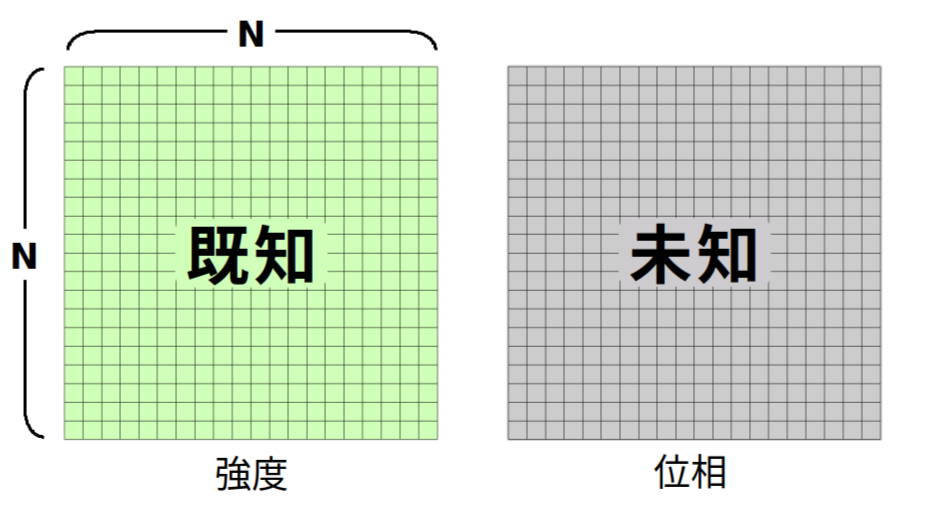
\includegraphics[width=11cm]{phase_retrieval_problem.png}
\caption{位相回復問題}
\label{fig:phase_retrieval_problem}
\end{figure}

\begin{figure}[!ht]
\centering
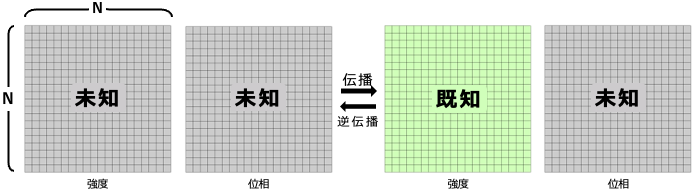
\includegraphics[width=13cm]{phase_retrieval_policy.png}
\caption{位相回復法の方針}
\label{fig:phase_retrieval_policy}
\end{figure}

以下では、代表的な解法を紹介し、続いてそれらを用いた天文用Wolterミラーの波面に対する位相回復法の検討・シミュレーションを行う。


\clearpage
% ================================================== %
% section
% ================================================== %
\newpage

\section{孤立条件の利用}
\label{chap3_solitude_introduction}
主にCDI(コヒーレント回折イメージング)の文脈において、波動場が到達しない領域を定数0として与えることで、未知数をの総数を激減させるという方法が多く取られる。
CDIとは、図\ref{fig:cdi_schematic}に示すように、サンプルに集光ビームを照射し、その回折像を見ることでそのサンプルの内部構造を解析する方法である。

\begin{figure}[!ht]
\centering
\includegraphics[width=12cm]{cdi_schematic.png}
\caption{コヒーレント回折イメージングの概要}
\label{fig:cdi_schematic}
\end{figure}

位相回復法によってディテクターでの位相およびサンプル面における位相・強度を求めることで、サンプル各点における透過率を求めることが目標となる。
このような系においては、カメラの画素をより細かく取ることにより、対応するサンプル面での領域がサンプルより大きく広がるため、この領域には波面が存在しないという仮定を用いて回復計算を行うことができる。
本研究で対象とするWolterミラーについても、回復の対象である輪帯状でかつ細い波面の面積が下流端開口面全体に対して非常に小さく、同様の方法が有効である可能性がある。
この方針に則って、位相回復計算を行う最もシンプルなアルゴリズムがBIO(Basic Input-Output) Algorithmである。
疑似コードをAlgorithm\ref{alg:bio}に示す。

\newcommand{\pos} {
    \mathbf{r}
}
\newcommand{\rpos} {
    \mathbf{q}
}

\begin{algorithm}                      
\caption{BIO Algorithm}         
\label{alg:bio}                          
\begin{algorithmic}
    \STATE $\phi_0(\pos)$
      = $\begin{cases}
        \mathrm{rand} & (\pos \in S) \\
        0 & (\pos \notin S)
      \end{cases}$
    \FOR{n = 0 \ldots N-1}
    \STATE $\Psi_n(\rpos) = \mathcal F [\phi_n(\pos)]$
    \STATE $\Psi_{n+1}(\rpos) = \sqrt{I(\rpos)} \exp \left( i \arg \Psi_n(\rpos) \right)$ 
    \STATE $\phi_n'(\pos) = \mathcal F^{-1} [\Psi_{n+1}(\rpos)]$
    \STATE $\phi_{n+1}(\pos)
      = \begin{cases}
          \phi_n'(\pos) & (\pos \in S) \\
          0 & (\pos \notin S)
      \end{cases}$
    \ENDFOR
\end{algorithmic}
\end{algorithm}

これを改良し、サポートによる射影を弱めることで収束性を高めたのが、HIO(Hybrid Input-Output) Algorithmである。
疑似コードはAlgorithm\ref{alg:hio}のようになる。

\begin{algorithm}                      
\caption{HIO Algorithm}         
\label{alg:hio}                          
\begin{algorithmic}
    \STATE $\phi_0(\pos)$
      = $\begin{cases}
        \mathrm{rand}(0,1) & (\pos \in S) \\
        0 & (\pos \notin S)
      \end{cases}$
    \FOR{n = 0 \ldots N-1}
    \STATE $\Psi_n(\rpos) = \mathcal F [\phi_n(\pos)]$
    \STATE $\Psi_{n+1}(\rpos) = \sqrt{I(\rpos)} \exp \left( i \arg \Psi_n(\rpos) \right)$ 
    \STATE $\phi_n'(\pos) = \mathcal F^{-1} [\Psi_{n+1}(\rpos)]$
    \STATE $\phi_{n+1}(\pos)
      = \begin{cases}
          \phi_n'(\pos) & (\pos \in S) \\
          \phi_n(\pos) - \beta \phi_n'(\pos) & (\pos \notin S)
      \end{cases}$
    \ENDFOR
\end{algorithmic}
\end{algorithm}

位相回復計算が収束するかどうかを決める最大の要因の1つが、オーバーサンプリング比、つまり試料に対してどれだけ大きな領域を取って計算できるかということである。
これは、カメラの空間分解能によって決まる。
位相回復計算が収束するために必要な最低限の条件として、FFTで結ばれる関係式の数が未知数の数を上回らなければならない。
Friedel則による対称性などを考慮すると、取得する総ピクセル数が回復する試料のピクセル数の2倍になっていなければいけないことになる。\cite{Latychevskaia2018}
実際にはノイズが乗ったり、直接通過する光が入射しないようにビームストップを配置したりといった事情から、2倍より大きくなければならない。

\clearpage
% ================================================== %
% section
% ================================================== %
\newpage

\section{タイコグラフィ法}
\label{chap3_ptychography_introduction}
\subsection{タイコグラフィ法の概要}
\ref{chap3_solitude_introduction}節では1枚の画像に対して孤立条件から冗長性を確保して位相回復を行ったが、タイコグラフィ法では光学系に徐々に変化を与えながら、多数の画像を撮影することによって冗長性を確保する。
図\ref{fig:ptychography_schematic}にその概要を示す。

\begin{figure}[!ht]
\centering
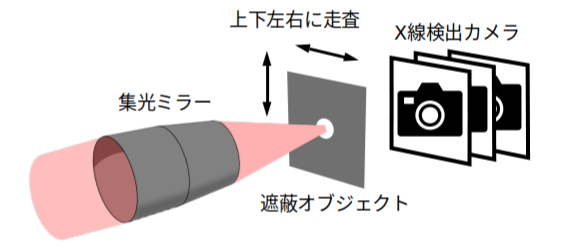
\includegraphics[width=12cm]{ptychography_schematic.png}
\caption{タイコグラフィ法の概要}
\label{fig:ptychography_schematic}
\end{figure}

集光ミラーに設計時に想定された光源からの入射光を入れ、その焦点面にオブジェクトを差し入れる。
このオブジェクトによって変化を受けた波面がさらに下流側に設置されたカメラによって撮影される。
これを、オブジェクトの位置を焦点面内で鉛直および水平方向に走査しながら多数の画像を撮影することで、冗長性を確保するという寸法である。
用いるオブジェクトは大きく分けて2種類ある。
1つはガラスなどの透過性を持つ物体の厚みに適当なパターンを与えた試料をオブジェクトとするものである。
物体の厚みを位置によって変えることで、それに応じて波面の位相の進み量に差が生じる。
試料の作製については、SiO2のエッチングによるパターニングなどが知られている。\cite{Godden2016}
この方法は、タイコグラフィによるミラー評価だけでなく、試料そのものを評価するタイコグラフィ顕微鏡としても利用できる。
もう1つは、ビームを完全に遮蔽できるような金属板に適当な穴を開けて作られるオブジェクトである。
焦点面における波面は完全に遮蔽される部分と完全に透過される部分の2つに分かれ、透過した波面の穴のエッジで回折した光が下流側のカメラに入射する。
これらのオブジェクトを焦点面内で走査し、各位置に対する回折光を

竹尾らは、ピンホール(1つの円形の穴)を開けた板をオブジェクトとして利用し、ピンホールのエッジをなぞるように走査する方法でタイコグラフィを行い、ミラー内面形状の評価に成功している。
ピンホールを用いた方法では、ミラーの内側で反射せず直接通過した光を処理することが位相パターンをつけた試料より容易である。

\subsection{PIE}
位相回復法は元来、X線顕微鏡として利用されたため、回復の対象はサンプル(オブジェクト)であった。
その最も簡単なタイコグラフィのアルゴリズムがPIE(Ptychography Iterative Engine)である。
これは、照明関数は既知であるとして与え、オブジェクトのみ回復計算を行うアルゴリズムである。
PIEの疑似コードをAlgorighm\ref{alg:pie}に示す。

\begin{algorithm}                      
\caption{PIE Algorithm}         
\label{alg:pie}                          
\begin{algorithmic}
    \STATE $O_0(\pos) = \mathrm{rand}(0,1) \exp(i \mathrm{rand}(0,1) )$
    \FOR{n = 0 \ldots N-1}
      \FOR{j = 0 \ldots M-1}
        \STATE $\psi(\pos_j) = P(\pos) O_n(\pos_j + \pos)$
        \STATE $\Psi(\rpos) = \mathcal F [\psi(\pos)]$
        \STATE $\Psi'(\rpos) = \sqrt{I_j(\rpos)} \exp\left( i \arg \psi(\pos) \right)$ 
        \STATE $\psi'(\pos) = \mathcal F^{-1} [\Psi'(\rpos)]$
        \STATE $O_{n+1}(\pos + \pos_j)'
          = O_n(\pos + \pos_j) 
          + \frac{P_n^*(\pos)}{|P(\pos)|^2+\varepsilon} \left( \psi_n'(\pos) - \psi_n(\pos) \right)$
      \ENDFOR
    \ENDFOR
\end{algorithmic}
\end{algorithm}

逆空間で拘束を掛け、実空間に戻したあとで、オブジェクトを更新する。
オブジェクトの更新則としてシンプルなのは$\psi(\pos_j) = P(\pos) O_n(\pos_j + \pos)$としたのに対応させて$O_{n+1}(\pos_j + \pos) = \frac{\psi'(\pos_j)}{P(\pos)}$とする方法である。
しかし、これは除算に際して発散が起こる可能性があり、実用上大きな問題を孕んでいる。
これを、式\ref{eqn:object_update_derivation}のように変形する。
\begin{eqnarray}
O_{n+1}(\pos_j + \pos)
  &=& \frac{\psi'(\pos_j)}{P(\pos)} \nonumber \\
  &=& \left( O_n(\pos_j + \pos) - \frac{\psi(\pos_j)}{P(\pos)} \right) + \frac{\psi'(\pos_j)}{P_n(\pos)} \nonumber \\
  &=& O_n(\pos_j + \pos) + \frac{1}{P(\pos)} \left( \psi'(\pos_j) - \psi(\pos_j) \right) \label{eqn:object_update_derivation}
\end{eqnarray}

これを一般化して文字を置き換えると、式\ref{eqn:object_update_simplified}のように書ける。
\begin{equation}
\label{eqn:object_update_simplified}
  O_{n+1}(\pos_j + \pos) = O_n(\pos_j + \pos) + w \Delta\psi(\pos)
\end{equation}
この更新の重み$w$を変えることで、アルゴリズムの改善を図る。
発散を回避するため、重みの分母を実数化して微小な定数$\varepsilon$を足して式\ref{eqn:pie_object_update_weight}のように重みを定めたのがAlgorithm\ref{alg:pie}に示したPIEのアルゴリズムである。
\begin{equation}
  \label{eqn:pie_object_update_weight}
  w = \frac{P*(\pos)}{\left| P(\pos) \right|^2 + \varepsilon}
\end{equation}

\subsection{rPIE}
PIEがオブジェクトのみ回復を行っていたのに対して、照明関数も未知として回復計算を行うのがePIE(exteded PIE)である。
ePIEでは式\ref{eqn:pie_object_update_weight}のように定数で発散を回避するのではなく、式\ref{eqn:epie_object_update_weight}のように絶対値の2乗の最大値を取る。
また、更新係数にハイパーパラメタ$\alpha$を掛けることで収束性を上げることができることが知られている。
\begin{equation}
  \label{eqn:epie_object_update_weight}
  w = \alpha \frac{P_n*(\pos)}{\max \left| P_n(\pos) \right|^2}
\end{equation}
ePIEでは照明関数も更新しなければいけないが、これはオブジェクトの更新と同様に式\ref{eqn:epie_probe_update}のように行われる。
\begin{equation}
\label{eqn:epie_probe_update}
  P_{n+1}(\pos) 
  = P_n(\pos) 
  + \beta \frac{O_n*(\pos_j + \pos)}{\max \left| O_n(\pos_j + \pos) \right|^2} \Delta\psi(\pos)
\end{equation}

ePIE(式\ref{eqn:epie_object_update_weight})のように最大値を取る方法に対して、各点での絶対値の2乗とその最大値で重み付き平均を取って分母とするのがrPIE(regularized PIE)である。
更新式は式\ref{eqn:rpie_object_update}および式\ref{eqn:rpie_probe_update}に示す通りである。
rPIEはほとんどePIEの一般化になっている。
\begin{eqnarray}
  O_{n+1}(\pos_j + \pos) &=& O_n(\pos_j + \pos) 
    + \frac{P_n*(\pos_j + \pos)}
      {\alpha \max \left| P_n(\pos) \right|^2 + (1-\alpha) \left| P_n(\pos) \right|^2}
    \Delta\psi(\pos) \label{eqn:rpie_object_update} \\
  P_{n+1}(\pos) &=& P_n(\pos) 
    + \frac{O_n*(\pos_j + \pos)}
      {\beta \max \left| O_n(\pos_j + \pos) \right|^2 + (1-\beta) \left| O_n(\pos_j + \pos) \right|^2}
    \Delta\psi(\pos) \label{eqn:rpie_probe_update}
\end{eqnarray}

rPIEのアルゴリズムをAlgorithm\ref{alg:rpie}に示す。

\begin{algorithm}                      
\caption{rPIE Algorithm}         
\label{alg:rpie}                          
\begin{algorithmic}
    \STATE $O_0(\pos) = \mathrm{rand}(0,1) \exp(i \mathrm{rand}(0,1) )$
    \STATE $P_0(\pos) = \mathrm{rand}(0,1) \exp(i \mathrm{rand}(0,1) )$
    \FOR{n = 0 \ldots N-1}
      \FOR{j = 0 \ldots M-1}
        \STATE $\psi(\pos_j) = P_n(\pos) O(\pos_j + \pos)$
        \STATE $\Psi(\rpos) = \mathcal F [\psi(\pos)]$
        \STATE $\Psi'(\rpos) = \sqrt{I_j(\rpos)} \exp\left( i \arg \psi(\pos) \right)$ 
        \STATE $\psi'(\pos) = \mathcal F^{-1} [\Psi'(\rpos)]$
        \STATE $O_{n+1}(\pos_j + \pos) 
          = O_n(\pos_j + \pos) + \frac{P_n*(\pos_j + \pos)}
          {\alpha \max \left| P_n(\pos) \right|^2 + (1-\alpha) \left| P_n(\pos) \right|^2}
          \Delta\psi(\pos)$
        \STATE $P_{n+1}(\pos)
          = P_n(\pos) + \frac{O_n*(\pos_j + \pos)}
          {\beta \max \left| O_n(\pos_j + \pos) \right|^2 + (1-\beta) \left| O_n(\pos_j + \pos) \right|^2}
          \Delta\psi(\pos)$
      \ENDFOR
    \ENDFOR
\end{algorithmic}
\end{algorithm}

タイコグラフィ法においても、走査ステップを変えることで回復領域の重なり具合が変化し、この比(オーバーサンプリング比)が収束性を左右する。
ステップが小さいほどオーバーサンプリング比は大きく収束性は高くなるが、その分必要な領域を走査し終えるのに必要な計測時間は増大してしまう。
Bunkらの検討によれば、オーバーサンプリング比が0.6程度が最適であるということが知られている。\cite{Bunk2008}

\subsection{Wolterミラー計測への適用}
Wolterミラー計測
ピンホールをオブジェクトとして用いるタイコグラフィ法でシミュレーションを行う。

\clearpage
% ================================================== %
% section
% ================================================== %
\newpage

\section{ディテクター走査による冗長性}

タイコグラフィ法ではオブジェクトを走査することで冗長性を確保したが、ディテクターを走査することで冗長性を確保する方法も知られている。

\begin{figure}[!ht]
\centering
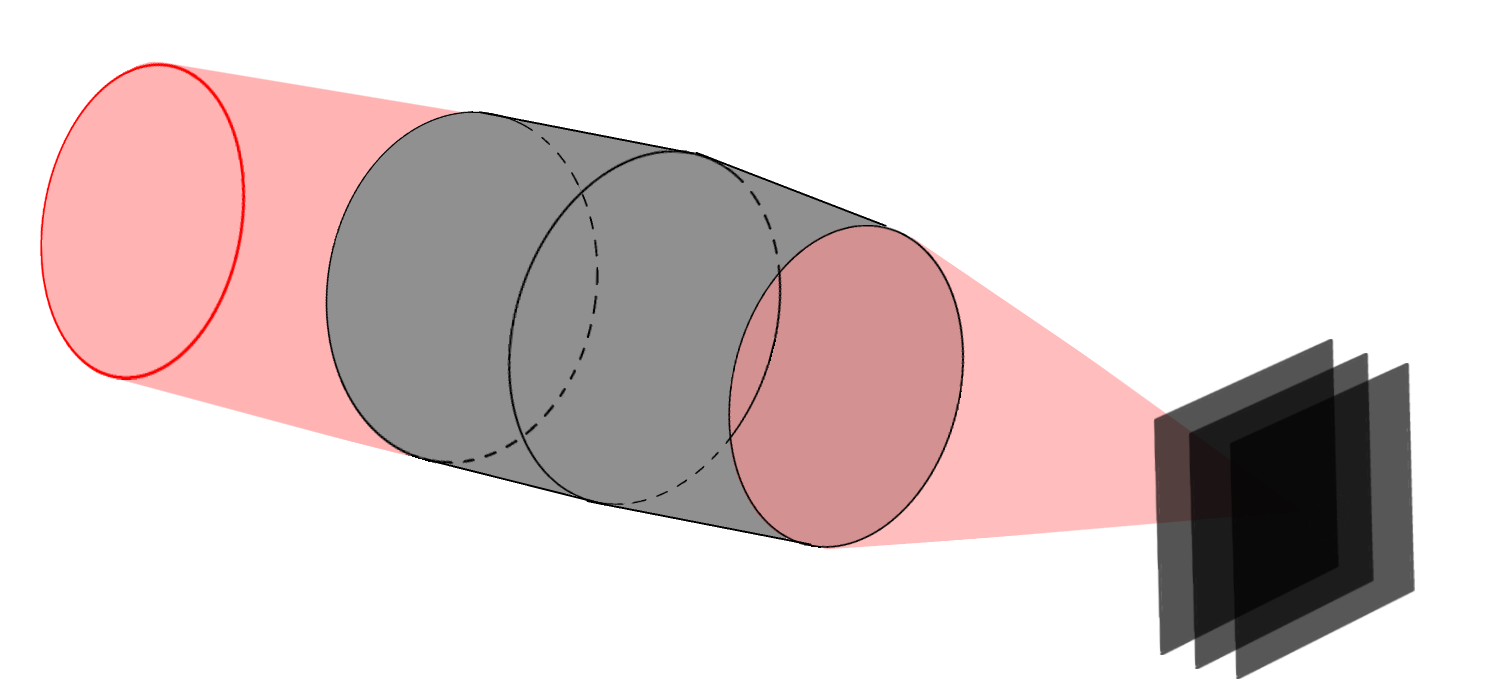
\includegraphics[width=12cm]{detector_scanning_schematic.png}
\caption{ディテクターを走査する方法の概要}
\label{fig:detector_scanning_schematic}
\end{figure}


\clearpage
% ================================================== %
% section
% ================================================== %
\newpage

\section{下流端開口走査による冗長性}

オブジェクトを走査する位置を焦点面ではなく集光素子の開口直後とするTransverse Translation法がBradyらによって提案されている。\cite{Brady2009}
これは図\ref{fig:transverse_schematic}に示すように、焦点面を操作するタイコグラフィ法同様にオブジェクトを集光素子の開口で走査し、その回折像を下流側のカメラで撮影するという方法である。

\begin{figure}[!ht]
\centering
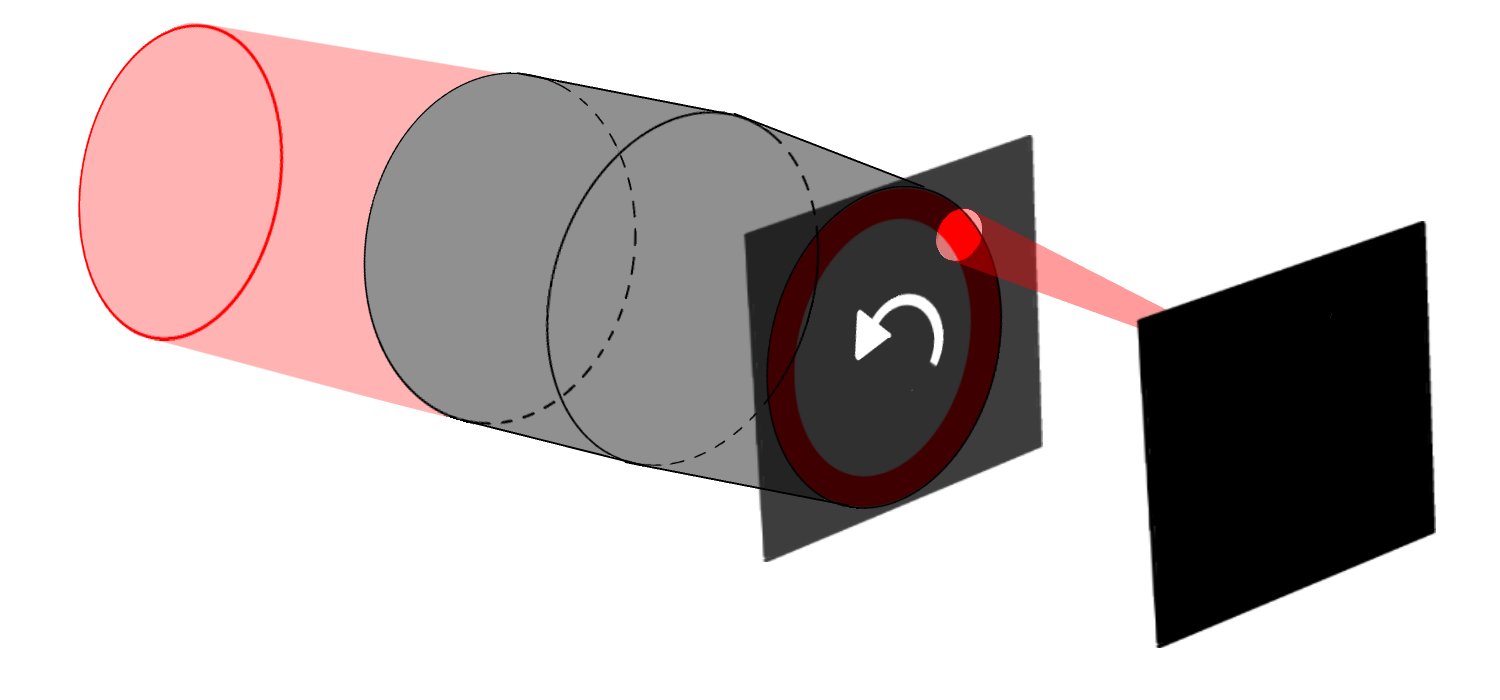
\includegraphics[width=12cm]{transverse_schematic.png}
\caption{Transverse Translation Diversityの概要}
\label{fig:transverse_schematic}
\end{figure}

計算アルゴリズム自体は基本的にはタイコグラフィ法と同様にすればよい。
タイコグラフィ法と構成が異なるため、同じ装置・素子に対して計算条件や分解能が異なる。

\subsection{対称性}

\clearpage
% ================================================== %
% section
% ================================================== %
\newpage


\section{結論}
\label{chap3_conclusion}
結論を述べる。




%%%%%%%%%%%%%%%%%%%%%%%%%%%%%%%%%%%%%%%%%%%%%%%%%%%%%%%%%%%%%%%%%%%%%%%%%%%%%
%%% Local Variables:
%%% mode: katex
%%% TeX-master: "../thesis"
%%% End:
